% Builds every paper figure as its own page for export (make figures-export).
% Captions and labels are dropped; the figures themselves are unchanged.
\documentclass[tikz,border=6pt]{standalone}
\usepackage[T1]{fontenc}
\usepackage{lmodern}
\usepackage{amsmath,amssymb,amsthm}
\usepackage{mathtools}
\usepackage[protrusion=true,expansion=false]{microtype}
\usepackage{booktabs}
\usepackage{tabularx}
\usepackage{graphicx}
\usepackage{xcolor}
\usepackage{enumitem}
\usepackage{tikz}
\usepackage{pgfplots}
\pgfplotsset{compat=1.18}
\usetikzlibrary{positioning,arrows.meta,fit,backgrounds,calc,shapes.geometric,decorations.pathreplacing,patterns}
\usepgfplotslibrary{groupplots}
% Categorical palette (fixed order) and neutrals for every figure.
\definecolor{cA}{HTML}{2A78D6}  % blue: representation / arithmetic
\definecolor{cB}{HTML}{EB6834}  % orange: instruction (hardware feature)
\definecolor{cC}{HTML}{1BAF7A}  % aqua: memory / layout
\definecolor{cD}{HTML}{EDA100}  % yellow: launch geometry
\definecolor{cE}{HTML}{6250D6}  % violet
\definecolor{inkS}{HTML}{52514E}
\definecolor{gridc}{HTML}{D9D8D3}
\definecolor{boxfill}{HTML}{F4F3EF}
\pgfplotsset{every axis/.append style={axis line style={inkS},tick style={inkS},
  major grid style={gridc},label style={font=\small},tick label style={font=\footnotesize},
  legend style={font=\footnotesize,draw=none,fill=none}}}

\newcommand{\FF}{\mathbb{F}}
\newcommand{\ZZ}{\mathbb{Z}}
\setlength{\textwidth}{159.2mm}
\renewenvironment{figure}[1][]{}{}
\renewcommand{\caption}[1]{}
\renewcommand{\label}[1]{}
\renewcommand{\centering}{}
\begin{document}
\begin{figure}[t]
\centering
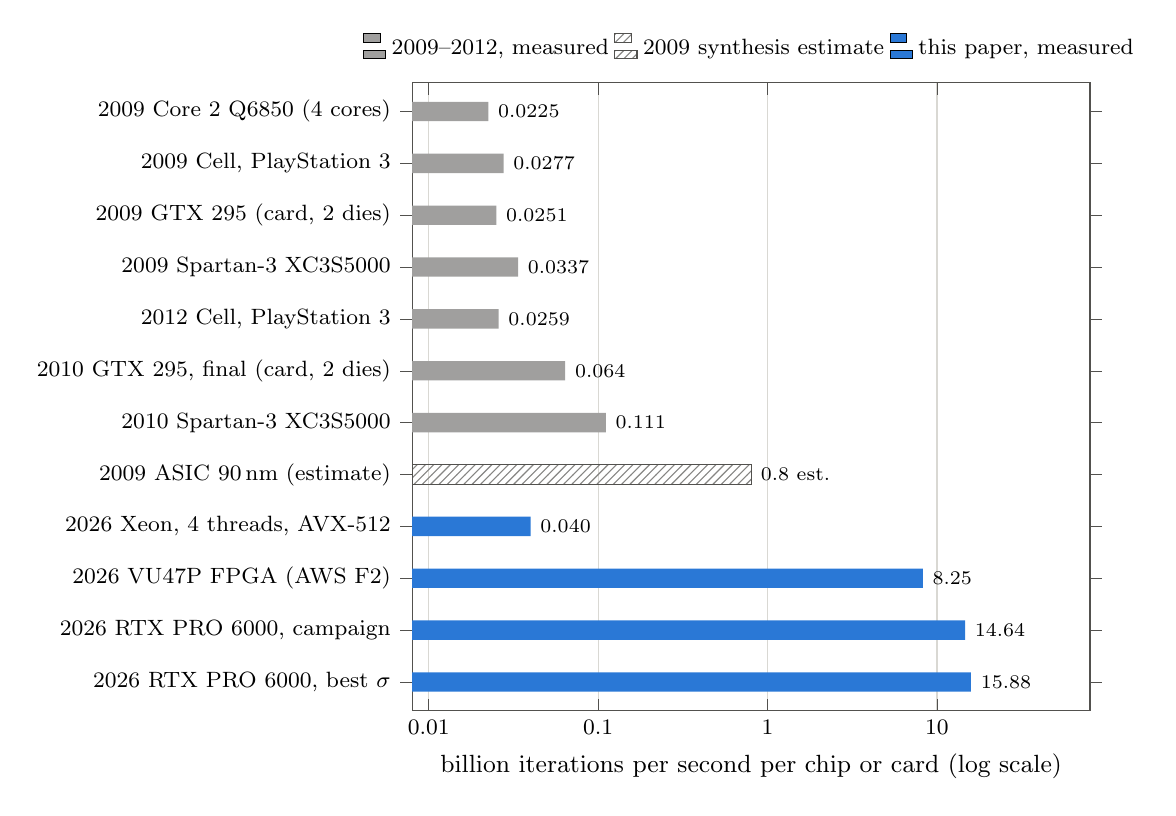
\begin{tikzpicture}
\begin{axis}[
  xbar, xmode=log, log basis x=10, log origin=infty,
  width=0.64\textwidth, height=0.6\textwidth,
  bar width=7pt, bar shift=0pt,
  xmin=0.008, xmax=80,
  xtick={0.01,0.1,1,10}, xticklabels={0.01,0.1,1,10},
  xlabel={billion iterations per second per chip or card (log scale)},
  symbolic y coords={core2,cell09,gtx09,sthreea,cell12,gtx10,sthreeb,asic,xeon,vu47p,pro6000c,pro6000b},
  ytick={core2,cell09,gtx09,sthreea,cell12,gtx10,sthreeb,asic,xeon,vu47p,pro6000c,pro6000b},
  yticklabels={
    {2009 Core 2 Q6850 (4 cores)},
    {2009 Cell, PlayStation 3},
    {2009 GTX 295 (card, 2 dies)},
    {2009 Spartan-3 XC3S5000},
    {2012 Cell, PlayStation 3},
    {2010 GTX 295, final (card, 2 dies)},
    {2010 Spartan-3 XC3S5000},
    {2009 ASIC 90\,nm (estimate)},
    {2026 Xeon, 4 threads, AVX-512},
    {2026 VU47P FPGA (AWS F2)},
    {2026 RTX PRO 6000, campaign},
    {2026 RTX PRO 6000, best $\sigma$},
  },
  y dir=reverse,
  xmajorgrids,
  enlarge y limits=0.05,
  nodes near coords,
  nodes near coords style={font=\scriptsize,color=black,anchor=west},
  point meta=explicit symbolic,
  legend style={at={(0.5,1.02)},anchor=south},
  legend columns=3,
  legend cell align=left,
]
\addplot[fill=inkS!55,draw=none] coordinates {
  (0.0225,core2) [0.0225] (0.0277,cell09) [0.0277] (0.0251,gtx09) [0.0251]
  (0.0337,sthreea) [0.0337] (0.0259,cell12) [0.0259] (0.064,gtx10) [0.064]
  (0.111,sthreeb) [0.111]};
\addlegendentry{2009--2012, measured}
\addplot[fill=white,draw=inkS,pattern=north east lines,pattern color=inkS!70] coordinates {(0.8,asic) [0.8 est.]};
\addlegendentry{2009 synthesis estimate}
\addplot[fill=cA,draw=none] coordinates {
  (0.040,xeon) [0.040] (8.25,vu47p) [8.25] (14.64,pro6000c) [14.64] (15.88,pro6000b) [15.88]};
\addlegendentry{this paper, measured}
\end{axis}
\end{tikzpicture}
\caption{ECC2K-130 rates, 2009--2012 against today, on one log scale
  (Tables~\ref{tab:history} and~\ref{tab:history-compare}). Each bar is
  one chip except the two GTX~295 bars, which are one card carrying two
  GPU dies, as their sources report them; per die they are half. One RTX~PRO~6000
  does the work of about 229 of the 2010 cards.}
\label{fig:history}
\end{figure}

\begin{figure}[t]
\centering
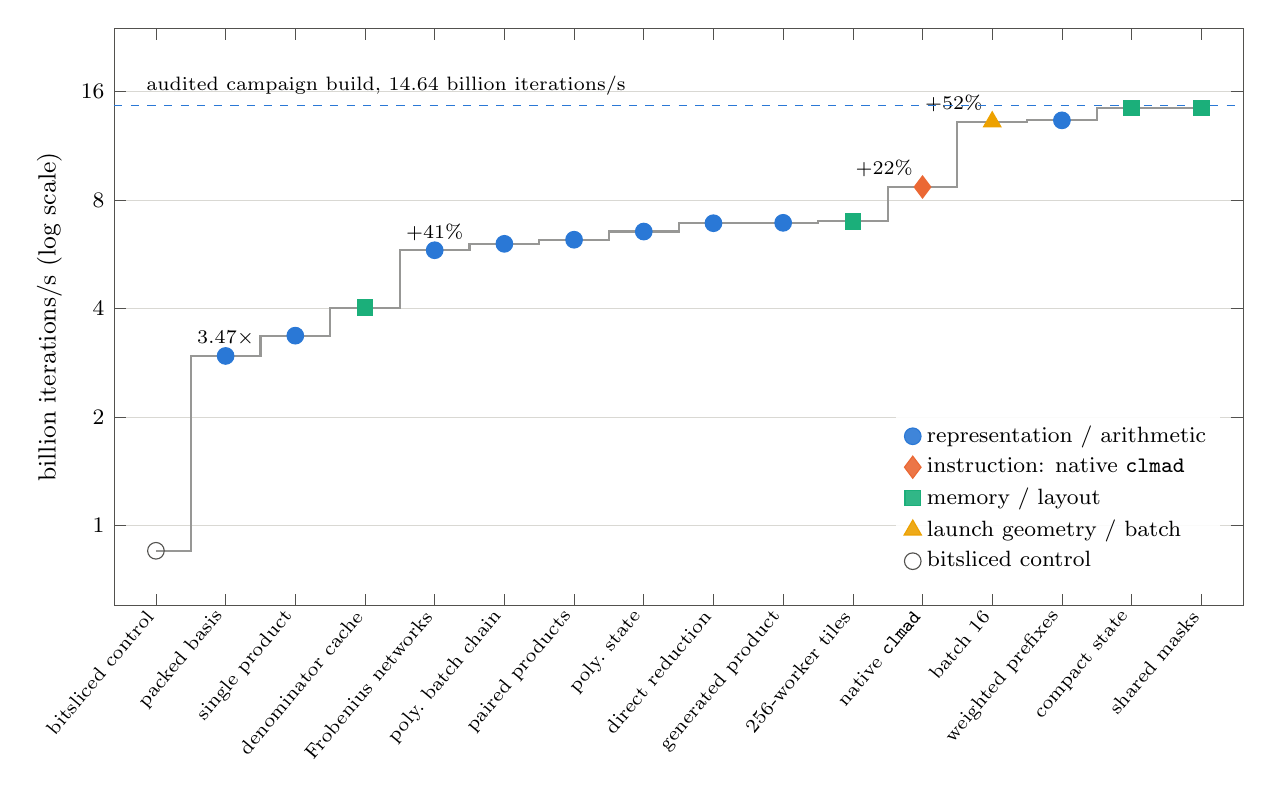
\begin{tikzpicture}
\begin{axis}[
  width=\textwidth, height=0.56\textwidth,
  ymode=log, log basis y=10,
  ymin=0.6, ymax=24,
  xmin=-0.6, xmax=15.6,
  ytick={1,2,4,8,16}, yticklabels={1,2,4,8,16},
  ylabel={billion iterations/s (log scale)},
  xtick={0,...,15},
  xticklabels={
    bitsliced control, packed basis, single product, denominator cache,
    Frobenius networks, poly.\ batch chain, paired products, poly.\ state,
    direct reduction, generated product, 256-worker tiles, native \texttt{clmad},
    batch 16, weighted prefixes, compact state, shared masks},
  x tick label style={rotate=50,anchor=east,font=\scriptsize},
  ymajorgrids,
  legend style={at={(0.98,0.04)},anchor=south east,fill=white,fill opacity=0.9,text opacity=1},
  legend cell align=left,
]
\addplot[inkS!60,thick,const plot mark mid,forget plot] coordinates {
  (0,0.852) (1,2.958) (2,3.367) (3,4.024) (4,5.811) (5,6.054) (6,6.215)
  (7,6.548) (8,6.906) (9,6.924) (10,6.995) (11,8.704) (12,13.206)
  (13,13.323) (14,14.403) (15,14.411)};
\addplot[only marks,mark=*,mark size=3pt,color=cA] coordinates {
  (1,2.958) (2,3.367) (4,5.811) (5,6.054) (6,6.215) (7,6.548) (8,6.906)
  (9,6.924) (13,13.323)};
\addlegendentry{representation / arithmetic}
\addplot[only marks,mark=diamond*,mark size=4pt,color=cB] coordinates {(11,8.704)};
\addlegendentry{instruction: native \texttt{clmad}}
\addplot[only marks,mark=square*,mark size=2.8pt,color=cC] coordinates {
  (3,4.024) (10,6.995) (14,14.403) (15,14.411)};
\addlegendentry{memory / layout}
\addplot[only marks,mark=triangle*,mark size=3.6pt,color=cD] coordinates {(12,13.206)};
\addlegendentry{launch geometry / batch}
\addplot[only marks,mark=o,mark size=3pt,color=inkS] coordinates {(0,0.852)};
\addlegendentry{bitsliced control}
\node[font=\scriptsize,anchor=south] at (axis cs:1,2.958) {$3.47\times$};
\node[font=\scriptsize,anchor=south] at (axis cs:4,5.811) {$+41\%$};
\node[font=\scriptsize,anchor=south east] at (axis cs:11,8.704) {$+22\%$};
\node[font=\scriptsize,anchor=south east] at (axis cs:12,13.206) {$+52\%$};
\draw[dashed,cA] (axis cs:-0.6,14.64) -- (axis cs:15.6,14.64)
  node[pos=0.02,anchor=south west,font=\scriptsize,color=black] {audited campaign build, 14.64 billion iterations/s};
\end{axis}
\end{tikzpicture}
\caption{The packed-backend ledger on one RTX~PRO~6000
  (Table~\ref{tab:ledger}), each step's candidate rate, with the marker
  showing what kind of change it was. No step changed the walk: the
  iteration function, the step count and the distinguished points are
  the same throughout. Steps are separate paired comparisons, not one
  chain, so the line joins candidates measured in different sessions.}
\label{fig:ledger}
\end{figure}

% Segment lengths are log10(factor) * \k cm, so widths multiply like the factors.
\begin{figure}[t]
\centering
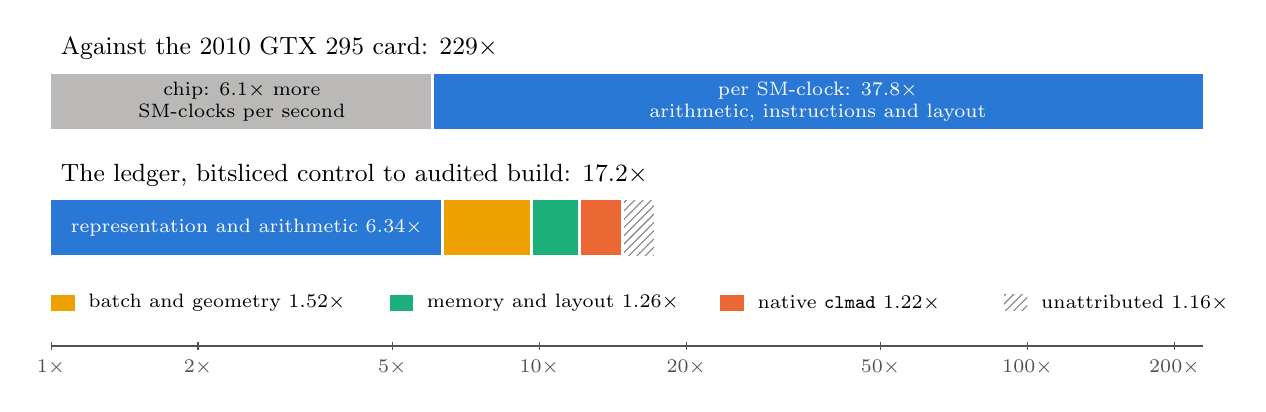
\begin{tikzpicture}[x=1cm,y=1cm,lab/.style={font=\scriptsize,align=center}]
\def\k{6.2}
% Row 1: 2010 GTX 295 -> RTX PRO 6000, 228.75x = SM-clocks 6.05x x per-SM-clock 37.8x
\pgfmathsetmacro{\p}{\k*log10(6.05)}
\pgfmathsetmacro{\q}{\k*log10(228.75)}
\node[anchor=south west,font=\small] at (0,2.62) {Against the 2010 GTX~295 card: $229\times$};
\fill[inkS!40] (0,1.85) rectangle (\p,2.55);
\fill[cA] (\p,1.85) rectangle (\q,2.55);
\draw[white,line width=1pt] (\p,1.85)--(\p,2.55);
\node[lab] at (\p/2,2.2) {chip: $6.1\times$ more\\SM-clocks per second};
\node[lab,text=white] at ({(\p+\q)/2},2.2) {per SM-clock: $37.8\times$\\arithmetic, instructions and layout};
% Row 2: ledger 0.852 -> 14.64, 17.17x
\pgfmathsetmacro{\a}{\k*log10(6.337)}
\pgfmathsetmacro{\b}{\a+\k*log10(1.523)}
\pgfmathsetmacro{\c}{\b+\k*log10(1.255)}
\pgfmathsetmacro{\d}{\c+\k*log10(1.224)}
\pgfmathsetmacro{\e}{\k*log10(17.17)}
\node[anchor=south west,font=\small] at (0,1.0) {The ledger, bitsliced control to audited build: $17.2\times$};
\fill[cA] (0,0.25) rectangle (\a,0.95);
\fill[cD] (\a,0.25) rectangle (\b,0.95);
\fill[cC] (\b,0.25) rectangle (\c,0.95);
\fill[cB] (\c,0.25) rectangle (\d,0.95);
\fill[white] (\d,0.25) rectangle (\e,0.95);
\fill[pattern=north east lines,pattern color=inkS!70] (\d,0.25) rectangle (\e,0.95);
\draw[white,line width=1pt] (\a,0.25)--(\a,0.95) (\b,0.25)--(\b,0.95) (\c,0.25)--(\c,0.95) (\d,0.25)--(\d,0.95);
\node[lab,text=white] at (\a/2,0.6) {representation and arithmetic $6.34\times$};
% Key for the narrow segments, in bar order.
\begin{scope}[shift={(0,-0.45)}]
\fill[cD] (0,0) rectangle (0.3,0.2); \node[lab,anchor=west] at (0.35,0.1) {batch and geometry $1.52\times$};
\fill[cC] (4.3,0) rectangle (4.6,0.2); \node[lab,anchor=west] at (4.65,0.1) {memory and layout $1.26\times$};
\fill[cB] (8.5,0) rectangle (8.8,0.2); \node[lab,anchor=west] at (8.85,0.1) {native \texttt{clmad} $1.22\times$};
\fill[pattern=north east lines,pattern color=inkS!70] (12.1,0) rectangle (12.4,0.2); \node[lab,anchor=west] at (12.45,0.1) {unattributed $1.16\times$};
\end{scope}
% log scale
\draw[inkS] (0,-0.9) -- (\q,-0.9);
\foreach \v in {1,2,5,10,20,50,100,200}
  \draw[inkS] ({\k*log10(\v)},-0.85) -- ({\k*log10(\v)},-0.95) node[below,font=\scriptsize] {$\v\times$};
\end{tikzpicture}
\caption{Where the speedup came from, on a log scale so that segment
  widths multiply. Top: against the 2010 GTX~295 card, about $6\times$ is a
  bigger, faster chip and about $38\times$ is per-SM-clock work. Bottom: the
  sixteen paired ledger steps grouped by kind (Figure~\ref{fig:ledger});
  their gains multiply to $14.8\times$ against the $17.2\times$ from the
  bitsliced control to the audited build, and the remaining $1.16\times$ is
  steps taken outside the ledger (launch shape, a compiler upgrade) and
  session-to-session drift. None of it changed the rho algorithm.}
\label{fig:gains}
\end{figure}

\begin{figure}[t]
\centering
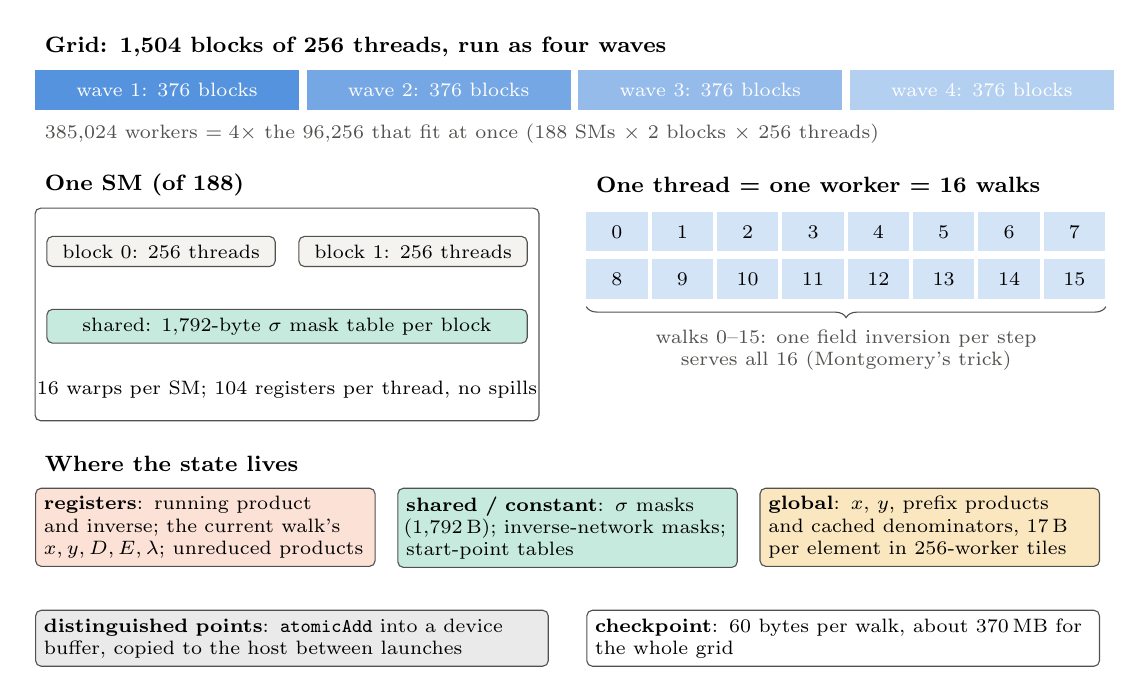
\begin{tikzpicture}[
  font=\scriptsize,x=1cm,y=1cm,
  box/.style={draw=inkS,rounded corners=2pt,fill=boxfill,align=center,inner sep=3pt},
  hdr/.style={font=\footnotesize\bfseries,anchor=west},
  arr/.style={-{Stealth[length=4pt]},inkS},
]
% ---- Row 1: grid and waves
\node[hdr] at (0,7.3) {Grid: 1{,}504 blocks of 256 threads, run as four waves};
\foreach \w in {0,1,2,3}{
  \fill[cA!\the\numexpr 80-\w*15\relax] ({\w*3.45},6.5) rectangle ({\w*3.45+3.35},7.0);
  \node[text=white] at ({\w*3.45+1.675},6.75) {wave \the\numexpr\w+1\relax: 376 blocks};
}
\node[anchor=west,text=inkS] at (0,6.2) {385{,}024 workers $=4\times$ the 96{,}256 that fit at once (188 SMs $\times$ 2 blocks $\times$ 256 threads)};
% ---- Row 2 left: one SM
\node[hdr] at (0,5.55) {One SM (of 188)};
\draw[inkS,rounded corners=2pt] (0,2.55) rectangle (6.4,5.25);
\node[box,minimum width=2.9cm] at (1.6,4.7) {block 0: 256 threads};
\node[box,minimum width=2.9cm] at (4.8,4.7) {block 1: 256 threads};
\node[box,fill=cC!25,minimum width=6.1cm] at (3.2,3.75) {shared: 1{,}792-byte $\sigma$ mask table per block};
\node at (3.2,2.95) {16 warps per SM; 104 registers per thread, no spills};
% ---- Row 2 right: one thread
\node[hdr] at (7.0,5.55) {One thread = one worker = 16 walks};
\foreach \s in {0,...,15}{
  \pgfmathsetmacro{\xx}{7.0+mod(\s,8)*0.83}
  \pgfmathsetmacro{\yy}{4.7-int(\s/8)*0.6}
  \fill[cA!20] (\xx,\yy) rectangle ({\xx+0.78},{\yy+0.5});
  \node[font=\scriptsize] at ({\xx+0.39},{\yy+0.25}) {\s};
}
\draw[decorate,decoration={brace,amplitude=4pt,mirror},inkS] (7.0,4.0) -- (13.6,4.0)
  node[midway,below=5pt,align=center] {walks 0--15: one field inversion per step\\serves all 16 (Montgomery's trick)};
% ---- Row 3: memory
\node[hdr] at (0,2.0) {Where the state lives};
\node[box,fill=cB!20,text width=4.1cm,anchor=north west,align=left] at (0,1.7)
  {\textbf{registers}: running product and inverse; the current walk's $x,y,D,E,\lambda$; unreduced products};
\node[box,fill=cC!25,text width=4.1cm,anchor=north west,align=left] at (4.6,1.7)
  {\textbf{shared / constant}: $\sigma$ masks (1{,}792\,B); inverse-network masks; start-point tables};
\node[box,fill=cD!25,text width=4.1cm,anchor=north west,align=left] at (9.2,1.7)
  {\textbf{global}: $x$, $y$, prefix products and cached denominators, 17\,B per element in 256-worker tiles};
\node[box,fill=inkS!12,text width=6.3cm,anchor=north west,align=left] at (0,0.15)
  {\textbf{distinguished points}: \texttt{atomicAdd} into a device buffer, copied to the host between launches};
\node[box,fill=white,text width=6.3cm,anchor=north west,align=left] at (7.0,0.15)
  {\textbf{checkpoint}: 60 bytes per walk, about 370\,MB for the whole grid};
\end{tikzpicture}
\caption{Anatomy of the audited $\sigma$-walk kernel on the RTX~PRO~6000.
  Each thread owns 16 walks that share one field inversion per step;
  two 256-thread blocks fit per SM, and the 385{,}024-worker grid runs in
  four waves. The 1{,}024-step loop runs inside the kernel; every step
  streams each walk's compact state through global memory, and the
  distinguished-point buffer is drained between launches.}
\label{fig:kernel}
\end{figure}

\begin{figure}[t]
\centering
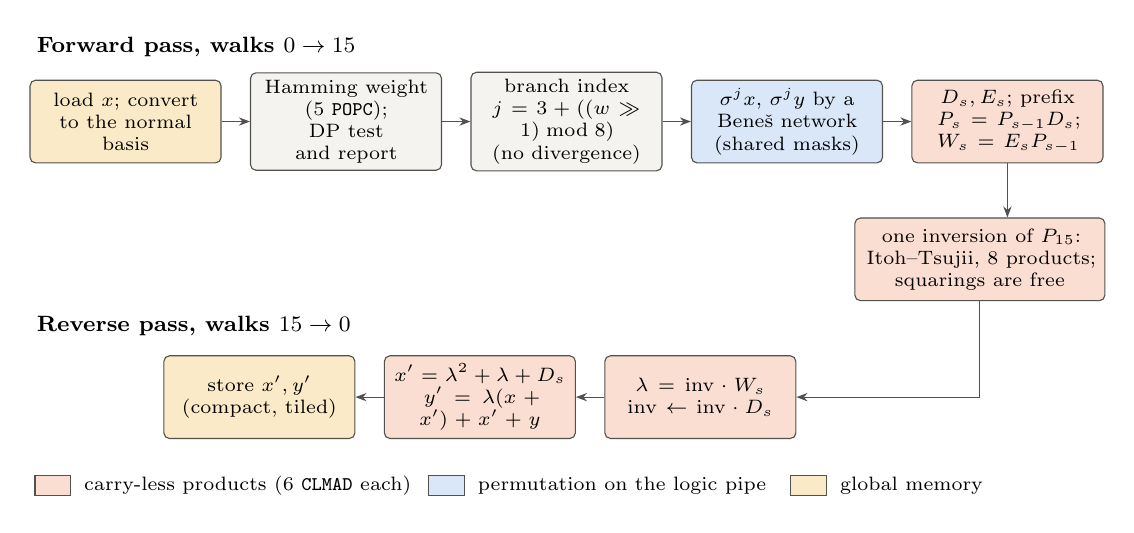
\begin{tikzpicture}[
  font=\scriptsize,x=1cm,y=1cm,
  st/.style={draw=inkS,rounded corners=2pt,fill=boxfill,align=center,inner sep=2.5pt,minimum height=1.05cm,text width=2.25cm},
  clm/.style={st,fill=cB!22},
  net/.style={st,fill=cA!18},
  mem/.style={st,fill=cD!22},
  arr/.style={-{Stealth[length=4pt]},inkS},
  lane/.style={font=\footnotesize\bfseries,anchor=west},
]
% Forward pass
\node[lane] at (-0.1,0.95) {Forward pass, walks $0\to15$};
\node[mem] (f1) at (1.15,0) {load $x$; convert\\to the normal\\basis};
\node[st]  (f2) at (3.95,0) {Hamming weight\\(5 \texttt{POPC});\\DP test and report};
\node[st]  (f3) at (6.75,0) {branch index\\$j=3+((w\gg1)\bmod8)$\\(no divergence)};
\node[net] (f4) at (9.55,0) {$\sigma^j x$, $\sigma^j y$ by a\\Bene\v{s} network\\(shared masks)};
\node[clm] (f5) at (12.35,0) {$D_s,E_s$; prefix\\$P_s=P_{s-1}D_s$;\\$W_s=E_sP_{s-1}$};
\foreach \a/\b in {f1/f2,f2/f3,f3/f4,f4/f5} \draw[arr] (\a)--(\b);
% Inversion
\node[clm,text width=3.0cm] (inv) at (12.0,-1.75) {one inversion of $P_{15}$:\\Itoh--Tsujii, 8 products;\\squarings are free};
\draw[arr] (f5) -- (f5|-inv.north);
% Reverse pass
\node[lane] at (-0.1,-2.6) {Reverse pass, walks $15\to0$};
\node[clm] (r1) at (8.45,-3.5) {$\lambda=\mathrm{inv}\cdot W_s$\\$\mathrm{inv}\leftarrow\mathrm{inv}\cdot D_s$};
\node[clm] (r2) at (5.65,-3.5) {$x'=\lambda^2+\lambda+D_s$\\$y'=\lambda(x+x')+x'+y$};
\node[mem] (r3) at (2.85,-3.5) {store $x',y'$\\(compact, tiled)};
\draw[arr] (inv.south) |- (r1.east);
\draw[arr] (r1)--(r2); \draw[arr] (r2)--(r3);
% Key
\begin{scope}[shift={(0,-4.75)}]
\fill[cB!22,draw=inkS] (0,0) rectangle (0.45,0.25); \node[anchor=west] at (0.5,0.125) {carry-less products (6 \texttt{CLMAD} each)};
\fill[cA!18,draw=inkS] (5.0,0) rectangle (5.45,0.25); \node[anchor=west] at (5.5,0.125) {permutation on the logic pipe};
\fill[cD!22,draw=inkS] (9.6,0) rectangle (10.05,0.25); \node[anchor=west] at (10.1,0.125) {global memory};
\end{scope}
\end{tikzpicture}
\caption{One step of the $\sigma$-walk for the 16 walks of a thread. The
  forward pass computes each walk's denominator and a running prefix
  product; one inversion of the final product then serves all 16; the
  reverse pass peels off each walk's inverse and finishes the affine
  addition. Per walk that is $4.81$ products of six \texttt{CLMAD} each plus
  a sixteenth of the inversion; everything else, including every
  Frobenius power, runs on the logic pipe.}
\label{fig:step}
\end{figure}

\begin{figure}[t]
\centering
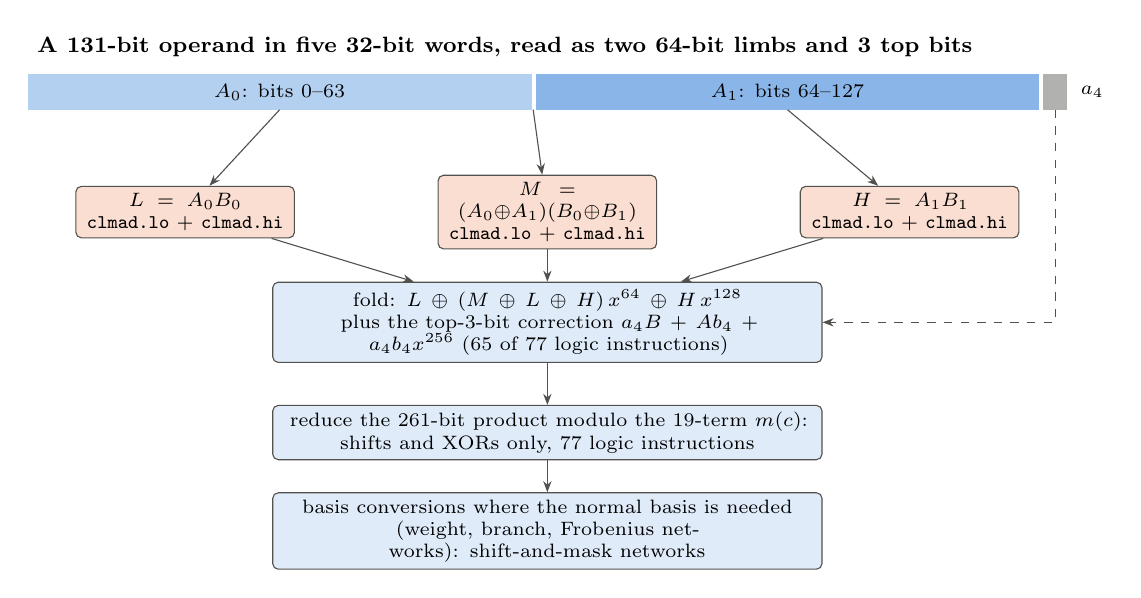
\begin{tikzpicture}[
  font=\scriptsize,
  arr/.style={-{Stealth[length=4pt]},inkS},
  leaf/.style={draw=inkS,rounded corners=2pt,fill=cB!22,align=center,inner sep=2.5pt,text width=2.6cm},
  alu/.style={draw=inkS,rounded corners=2pt,fill=cA!15,align=center,inner sep=2.5pt},
]
% operand
\node[anchor=west,font=\footnotesize\bfseries] at (0,4.35) {A 131-bit operand in five 32-bit words, read as two 64-bit limbs and 3 top bits};
\fill[cA!35] (0,3.55) rectangle (6.4,4.0);  \node at (3.2,3.775) {$A_0$: bits 0--63};
\fill[cA!55] (6.45,3.55) rectangle (12.85,4.0); \node at (9.65,3.775) {$A_1$: bits 64--127};
\fill[inkS!45] (12.9,3.55) rectangle (13.2,4.0); \node[anchor=west] at (13.25,3.775) {$a_4$};
% leaves
\node[leaf] (L) at (2.0,2.25) {$L=A_0B_0$\\\texttt{clmad.lo} + \texttt{clmad.hi}};
\node[leaf] (M) at (6.6,2.25) {$M=(A_0{\oplus}A_1)(B_0{\oplus}B_1)$\\\texttt{clmad.lo} + \texttt{clmad.hi}};
\node[leaf] (H) at (11.2,2.25) {$H=A_1B_1$\\\texttt{clmad.lo} + \texttt{clmad.hi}};
\draw[arr] (3.2,3.55) -- (L); \draw[arr] (6.42,3.55) -- (M); \draw[arr] (9.65,3.55) -- (H);
% fold
\node[alu,text width=6.8cm] (F) at (6.6,0.85) {fold: $L \oplus (M\oplus L\oplus H)\,x^{64} \oplus H\,x^{128}$\\
  plus the top-3-bit correction $a_4B + Ab_4 + a_4b_4x^{256}$ (65 of 77 logic instructions)};
\draw[arr] (L) -- (F); \draw[arr] (M) -- (F); \draw[arr] (H) -- (F);
\draw[arr,dashed] (13.05,3.55) -- (13.05,0.85) -- (F.east);
% reduction
\node[alu,text width=6.8cm] (R) at (6.6,-0.55) {reduce the 261-bit product modulo the 19-term $m(c)$:\\shifts and XORs only, 77 logic instructions};
\draw[arr] (F) -- (R);
\node[alu,text width=6.8cm] (C) at (6.6,-1.8) {basis conversions where the normal basis is needed\\(weight, branch, Frobenius networks): shift-and-mask networks};
\draw[arr] (R) -- (C);
\end{tikzpicture}
\caption{The packed 131-bit product. Three $64\times64$ carry-less leaves
  (six \texttt{CLMAD} instructions) form a one-level Karatsuba; the three
  top bits, the fold, the reduction and every basis change run on the
  logic pipe. On the RTX~PRO~6000 a \texttt{CLMAD} costs the issue time of
  $37.8$ logic instructions, so the split keeps only the six leaf products
  on the carry-less unit; on a B200 or H100, where it costs $2$--$3.8$,
  moving the correction and even the reduction onto \texttt{CLMAD} pays
  instead (Section~\ref{sec:blackwell-rates}).}
\label{fig:clmad}
\end{figure}

\begin{figure}[t]
\centering
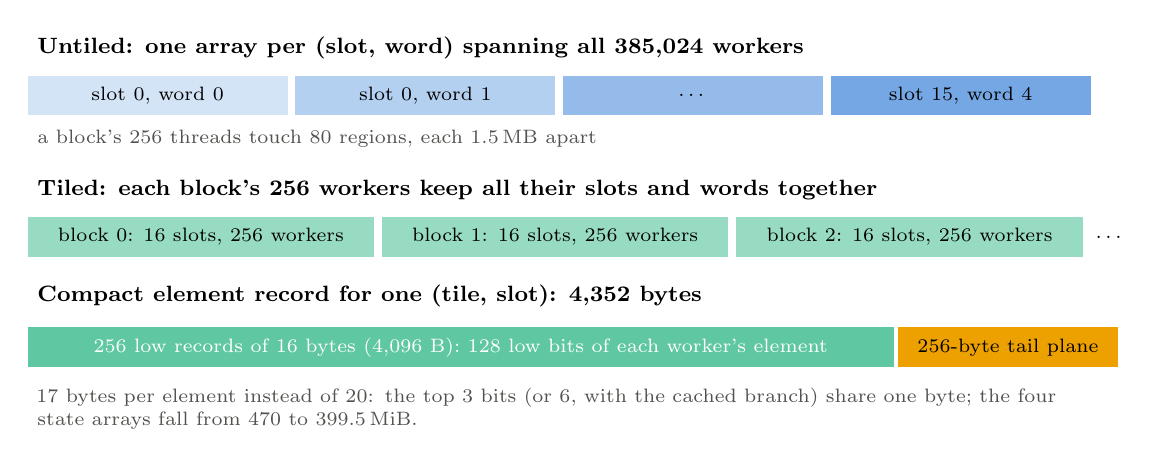
\begin{tikzpicture}[font=\scriptsize,x=1cm,y=1cm]
% Untiled
\node[anchor=west,font=\footnotesize\bfseries] at (0,3.45) {Untiled: one array per (slot, word) spanning all 385{,}024 workers};
\foreach \i/\t in {0/{slot 0, word 0},1/{slot 0, word 1},2/{\dots},3/{slot 15, word 4}}{
  \fill[cA!\the\numexpr 20+\i*15\relax] ({\i*3.4},2.6) rectangle ({\i*3.4+3.3},3.1);
  \node at ({\i*3.4+1.65},2.85) {\t};
}
\node[anchor=west,text=inkS] at (0,2.3) {a block's 256 threads touch 80 regions, each 1.5\,MB apart};
% Tiled
\node[anchor=west,font=\footnotesize\bfseries] at (0,1.65) {Tiled: each block's 256 workers keep all their slots and words together};
\foreach \b in {0,1,2}{
  \fill[cC!45] ({\b*4.5},0.8) rectangle ({\b*4.5+4.4},1.3);
  \node at ({\b*4.5+2.2},1.05) {block \b: 16 slots, 256 workers};
}
\node at (13.75,1.05) {\dots};
% Compact record
\node[anchor=west,font=\footnotesize\bfseries] at (0,0.3) {Compact element record for one (tile, slot): 4{,}352 bytes};
\fill[cC!70] (0,-0.6) rectangle (11.0,-0.1);
\node[text=white] at (5.5,-0.35) {256 low records of 16 bytes (4{,}096 B): 128 low bits of each worker's element};
\fill[cD] (11.05,-0.6) rectangle (13.85,-0.1);
\node at (12.45,-0.35) {256-byte tail plane};
\node[anchor=north west,text=inkS,align=left,text width=13.6cm] at (0,-0.75)
  {17 bytes per element instead of 20: the top 3 bits (or 6, with the cached branch) share one byte;
   the four state arrays fall from 470 to 399.5\,MiB.};
\end{tikzpicture}
\caption{How walk state is laid out in global memory. Tiling puts all of
  a block's state in one contiguous region while each warp still reads
  adjacent words ($+2.1\%$); the compact record then packs each 131-bit
  element into 17 bytes ($+6.3\%$). Neither changes a single bit of the
  walk.}
\label{fig:tiling}
\end{figure}

\begin{figure}[t]
\centering
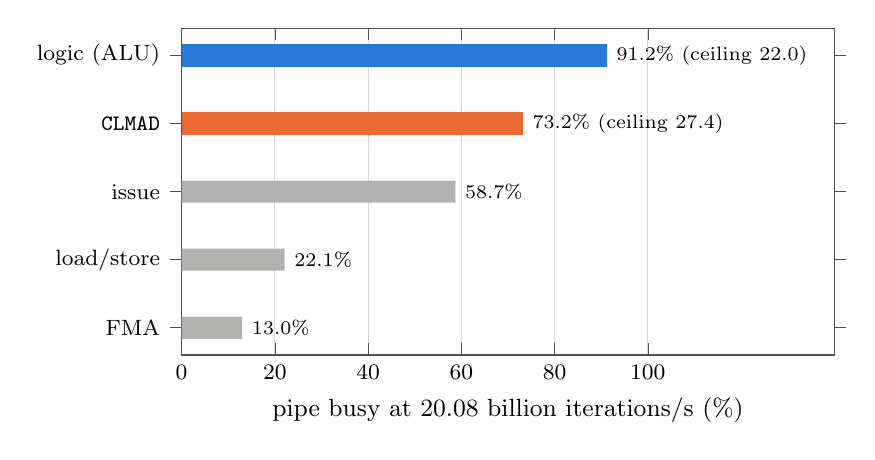
\begin{tikzpicture}
\begin{axis}[
  xbar, bar width=8pt, bar shift=0pt,
  width=0.62\textwidth, height=0.36\textwidth,
  xmin=0, xmax=140, xtick={0,20,...,100},
  xlabel={pipe busy at 20.08 billion iterations/s (\%)},
  symbolic y coords={alu,clmad,issue,lsu,fma},
  ytick={alu,clmad,issue,lsu,fma},
  yticklabels={logic (ALU),\texttt{CLMAD},issue,load/store,FMA},
  y dir=reverse, xmajorgrids,
  nodes near coords, nodes near coords style={font=\scriptsize,anchor=west},
  point meta=explicit symbolic,
]
\addplot[fill=cA,draw=none] coordinates {(91.2,alu) [91.2\% (ceiling 22.0)]};
\addplot[fill=cB,draw=none] coordinates {(73.2,clmad) [73.2\% (ceiling 27.4)]};
\addplot[fill=inkS!45,draw=none] coordinates {(58.7,issue) [58.7\%] (22.1,lsu) [22.1\%] (13.0,fma) [13.0\%]};
\end{axis}
\end{tikzpicture}
\caption{The roofline of Table~\ref{tab:roofline} as a picture: the logic
  pipe is the binding constraint for the table walk's arithmetic on the
  RTX~PRO~6000, with the carry-less unit second; memory and the FMA pipe
  are far from busy. In brackets, the rate at which each unit alone would
  saturate, in billions of iterations per second. Utilisation comes from
  dynamic instruction counts and measured pipe rates, not hardware
  counters (Section~\ref{sec:profiling}).}
\label{fig:roofline}
\end{figure}

\begin{figure}[t]
\centering
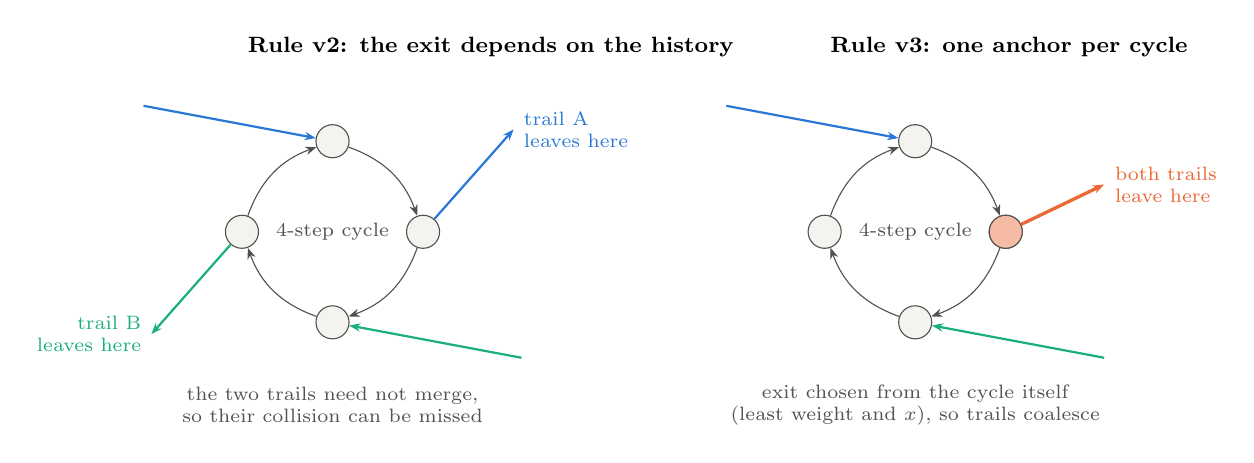
\begin{tikzpicture}[font=\scriptsize,
  pt/.style={circle,draw=inkS,fill=boxfill,inner sep=1.6pt,minimum size=0.42cm},
  anc/.style={pt,fill=cB!45},
  arr/.style={-{Stealth[length=4pt]},inkS},
  trA/.style={-{Stealth[length=4pt]},cA,thick},
  trB/.style={-{Stealth[length=4pt]},cC,thick},
]
\foreach \panel/\dx/\title in {0/0/{Rule v2: the exit depends on the history},1/7.4/{Rule v3: one anchor per cycle}}{
\begin{scope}[shift={(\dx,0)}]
\node[font=\footnotesize\bfseries,anchor=west] at (-1.2,2.35) {\title};
\foreach \i/\ang in {0/90,1/0,2/270,3/180}
  \node[pt] (c\panel\i) at (\ang:1.15) {};
\foreach \i/\j in {0/1,1/2,2/3,3/0}
  \draw[arr] (c\panel\i) to[bend left=25] (c\panel\j);
\node[font=\scriptsize,text=inkS] at (0,0) {4-step cycle};
\end{scope}}
% v2: two trails enter at different vertices and leave by different edges
\draw[trA] (-2.4,1.6) -- (c00);
\draw[trB] (2.4,-1.6) -- (c02);
\draw[trA] (c01) -- (2.3,1.3) node[right,align=left] {trail A\\leaves here};
\draw[trB] (c03) -- (-2.3,-1.3) node[left,align=right] {trail B\\leaves here};
\node[align=center,text=inkS] at (0,-2.2) {the two trails need not merge,\\so their collision can be missed};
% v3: both leave at the anchor (least key)
\node[anc] at (c11) {};
\draw[trA] (7.4-2.4,1.6) -- (c10);
\draw[trB] (7.4+2.4,-1.6) -- (c12);
\draw[trA,cB,very thick] (c11) -- (7.4+2.4,0.6) node[right,align=left] {both trails\\leave here};
\node[align=center,text=inkS] at (7.4,-2.2) {exit chosen from the cycle itself\\(least weight and $x$), so trails coalesce};
\end{tikzpicture}
\caption{Why the table walk's $20.08$ does not count. A table walk on
  Frobenius classes has short fruitless cycles that a trail must detect
  and leave. Under rule v2 the exit depended on how a trail arrived, so
  two trails entering the same cycle from different directions could
  leave by different edges and so fail to merge. Rule v3 confirms the cycle by
  walking it (at most eight raw steps) and leaves at one anchor chosen
  from the cycle's own points, so every trail entering it leaves the same
  way. The $\sigma$-walk has no fruitless cycles at all.}
\label{fig:cycles}
\end{figure}

\begin{figure}[t]
\centering
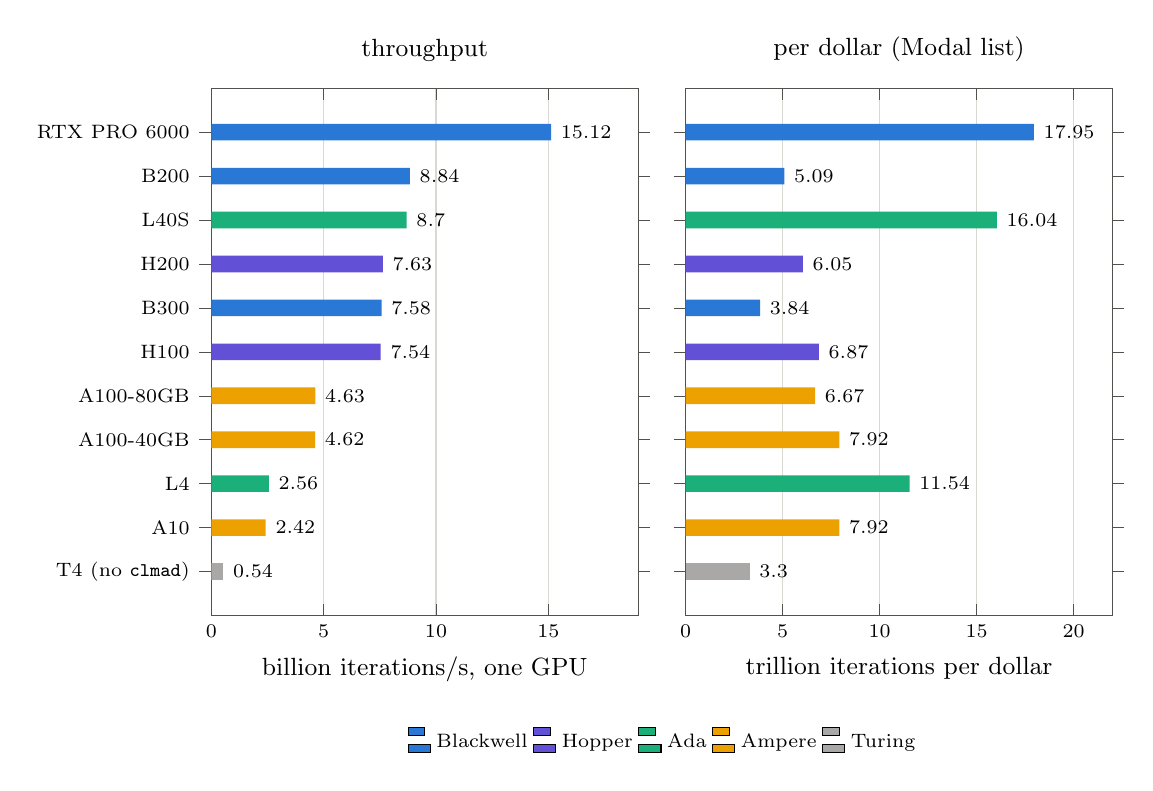
\begin{tikzpicture}
\begin{groupplot}[
  group style={group size=2 by 1, horizontal sep=0.6cm, yticklabels at=edge left},
  xbar, /pgf/bar width=6pt, /pgf/bar shift=0pt,
  width=0.44\textwidth, height=0.52\textwidth,
  symbolic y coords={p6000,b200,l40s,h200,b300,h100,a10080,a10040,l4,a10,t4},
  ytick={p6000,b200,l40s,h200,b300,h100,a10080,a10040,l4,a10,t4},
  yticklabels={RTX PRO 6000,B200,L40S,H200,B300,H100,A100-80GB,A100-40GB,L4,A10,T4 (no \texttt{clmad})},
  y dir=reverse,
  xmajorgrids, xmin=0,
  nodes near coords, nodes near coords style={font=\scriptsize,anchor=west},
  tick label style={font=\scriptsize},
]
\nextgroupplot[xmax=19, xlabel={billion iterations/s, one GPU}, title={\small throughput}]
\addplot[fill=cA,draw=none] coordinates {(15.116,p6000) (8.840,b200) (7.575,b300)};
\addplot[fill=cE,draw=none] coordinates {(7.632,h200) (7.540,h100)};
\addplot[fill=cC,draw=none] coordinates {(8.696,l40s) (2.561,l4)};
\addplot[fill=cD,draw=none] coordinates {(4.632,a10080) (4.618,a10040) (2.423,a10)};
\addplot[fill=inkS!50,draw=none] coordinates {(0.541,t4)};
\nextgroupplot[xmax=22, xlabel={trillion iterations per dollar}, title={\small per dollar (Modal list)},
  legend style={at={(-0.05,-0.2)},anchor=north,font=\scriptsize,draw=none},legend columns=5]
\addplot[fill=cA,draw=none] coordinates {(17.95,p6000) (5.09,b200) (3.84,b300)};
\addlegendentry{Blackwell}
\addplot[fill=cE,draw=none] coordinates {(6.05,h200) (6.87,h100)};
\addlegendentry{Hopper}
\addplot[fill=cC,draw=none] coordinates {(16.04,l40s) (11.54,l4)};
\addlegendentry{Ada}
\addplot[fill=cD,draw=none] coordinates {(6.67,a10080) (7.92,a10040) (7.92,a10)};
\addlegendentry{Ampere}
\addplot[fill=inkS!50,draw=none] coordinates {(3.30,t4)};
\addlegendentry{Turing}
\end{groupplot}
\end{tikzpicture}
\caption{The campaign's $\sigma$-walk on eleven GPUs, one survey run each
  with the same preset (Table~\ref{tab:survey}), by throughput and by
  iterations per dollar at Modal list price. The workstation Blackwell
  part leads on both; the data-centre Blackwell and Hopper parts run this
  integer-bound walk at about half its rate and a third of its value.}
\label{fig:gpus}
\end{figure}

\begin{figure}[t]
\centering
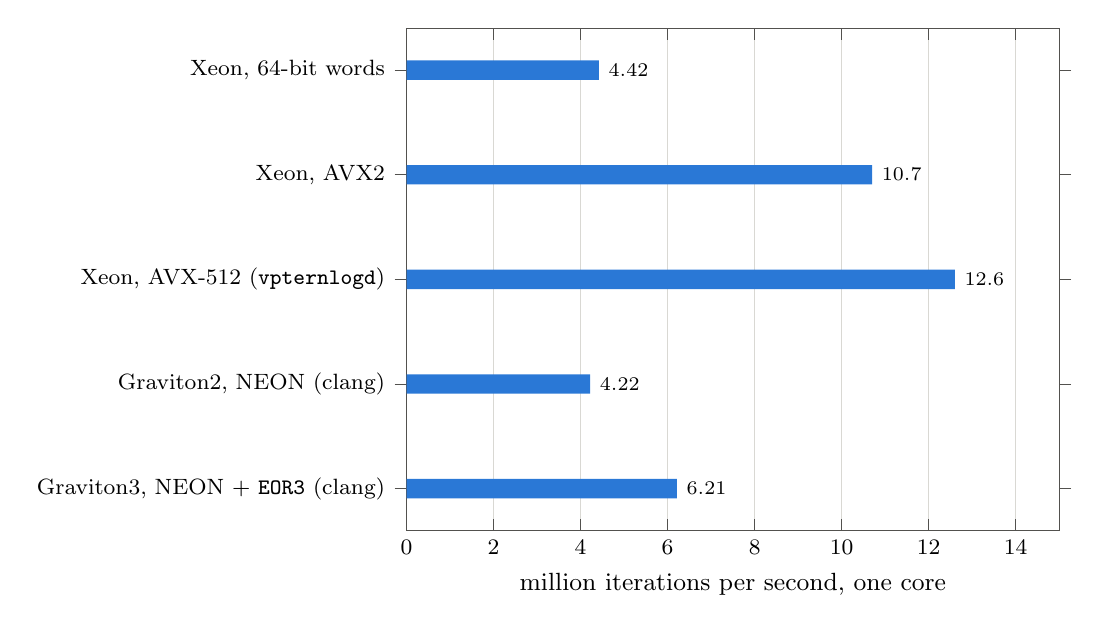
\begin{tikzpicture}
\begin{axis}[
  xbar, bar width=7pt, bar shift=0pt,
  width=0.62\textwidth, height=0.5\textwidth,
  xmin=0, xmax=15,
  xlabel={million iterations per second, one core},
  symbolic y coords={x64,xavx2,xavx512,g2,g3},
  ytick={x64,xavx2,xavx512,g2,g3},
  yticklabels={
    {Xeon, 64-bit words},
    {Xeon, AVX2},
    {Xeon, AVX-512 (\texttt{vpternlogd})},
    {Graviton2, NEON (clang)},
    {Graviton3, NEON + \texttt{EOR3} (clang)},
  },
  y dir=reverse,
  xmajorgrids,
  nodes near coords, nodes near coords style={font=\scriptsize,anchor=west},
  legend style={at={(0.5,-0.2)},anchor=north},
  legend columns=2,
  legend cell align=left,
]
\addplot[fill=cA,draw=none] coordinates {(4.42,x64) (10.7,xavx2) (12.6,xavx512)
  (4.220,g2) (6.214,g3)};
\end{axis}
\end{tikzpicture}
\caption{CPU rates per core by instruction set. Bitsliced rows are the
  campaign walk (Table~\ref{tab:cpu}); each step down a group adds one
  extension.}
\label{fig:cpu}
\end{figure}

\begin{figure}[t]
\centering
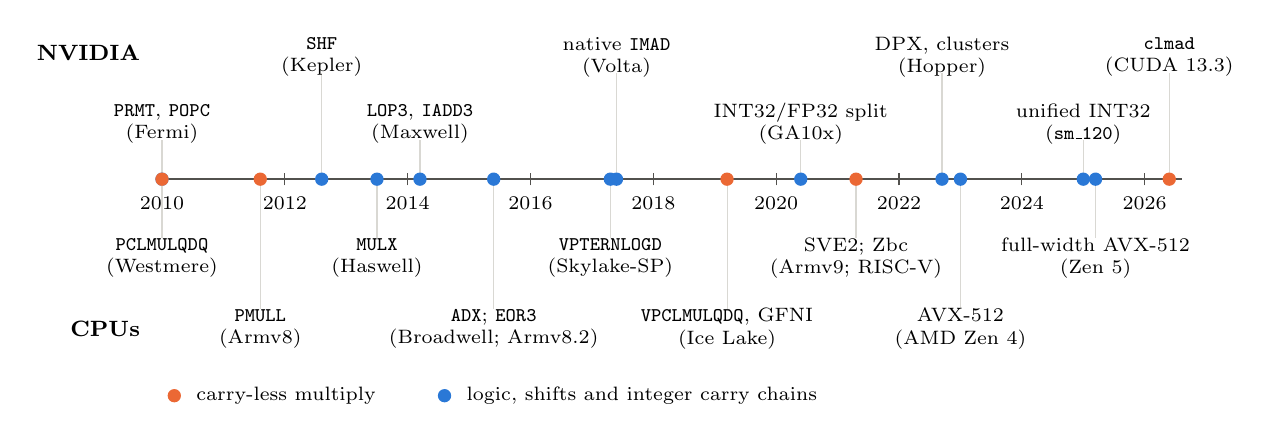
\begin{tikzpicture}[x=0.78cm,y=1cm,font=\scriptsize,
  ev/.style={circle,inner sep=1.7pt},
  lbl/.style={align=center,font=\scriptsize}]
% axis
\draw[inkS,thick] (0,0) -- (16.6,0);
\foreach \y in {0,2,...,16}{
  \draw[inkS] (\y,-0.08) -- (\y,0.08);
  \node[below,font=\scriptsize] at (\y,-0.1) {\the\numexpr2010+\y\relax};
}
\node[anchor=east,font=\footnotesize\bfseries] at (-0.2,1.6) {NVIDIA};
\node[anchor=east,font=\footnotesize\bfseries] at (-0.2,-1.9) {CPUs};
% GPU events (above)
\foreach \x/\h/\t/\c in {
  0/0.7/{\texttt{PRMT}, \texttt{POPC}\\(Fermi)}/cA,
  2.6/1.55/{\texttt{SHF}\\(Kepler)}/cA,
  4.2/0.7/{\texttt{LOP3}, \texttt{IADD3}\\(Maxwell)}/cA,
  7.4/1.55/{native \texttt{IMAD}\\(Volta)}/cA,
  10.4/0.7/{INT32/FP32 split\\(GA10x)}/cA,
  12.7/1.55/{DPX, clusters\\(Hopper)}/cA,
  15/0.7/{unified INT32\\(\texttt{sm\_120})}/cA,
  16.4/1.55/{\texttt{clmad}\\(CUDA 13.3)}/cB}{
  \draw[gridc] (\x,0) -- (\x,\h-0.2);
  \node[ev,fill=\c] at (\x,0) {};
  \node[lbl] at (\x,\h) {\t};
}
% CPU events (below)
\foreach \x/\h/\t/\c in {
  0/-1.0/{\texttt{PCLMULQDQ}\\(Westmere)}/cB,
  1.6/-1.9/{\texttt{PMULL}\\(Armv8)}/cB,
  3.5/-1.0/{\texttt{MULX}\\(Haswell)}/cA,
  5.4/-1.9/{\texttt{ADX}; \texttt{EOR3}\\(Broadwell; Armv8.2)}/cA,
  7.3/-1.0/{\texttt{VPTERNLOGD}\\(Skylake-SP)}/cA,
  9.2/-1.9/{\texttt{VPCLMULQDQ}, GFNI\\(Ice Lake)}/cB,
  11.3/-1.0/{SVE2; Zbc\\(Armv9; RISC-V)}/cB,
  13.0/-1.9/{AVX-512\\(AMD Zen 4)}/cA,
  15.2/-1.0/{full-width AVX-512\\(Zen 5)}/cA}{
  \draw[gridc] (\x,0) -- (\x,\h+0.25);
  \node[ev,fill=\c] at (\x,0) {};
  \node[lbl] at (\x,\h) {\t};
}
\node[ev,fill=cB] at (0.2,-2.75) {}; \node[anchor=west] at (0.4,-2.75) {carry-less multiply};
\node[ev,fill=cA] at (4.6,-2.75) {}; \node[anchor=west] at (4.8,-2.75) {logic, shifts and integer carry chains};
\end{tikzpicture}
\caption{When the instructions this arithmetic relies on arrived. Dates
  are first availability in a shipping product (Armv8 and Armv8.2 are
  architecture versions; Zbc is the ratification date). The GPU
  carry-less multiply arrived last of all, in 2026, which is why the
  ECC2K-130 GPU client is new work rather than a port.}
\label{fig:isa}
\end{figure}

% x: billion iterations per second, 0.37 cm per unit.
\begin{figure}[t]
\centering
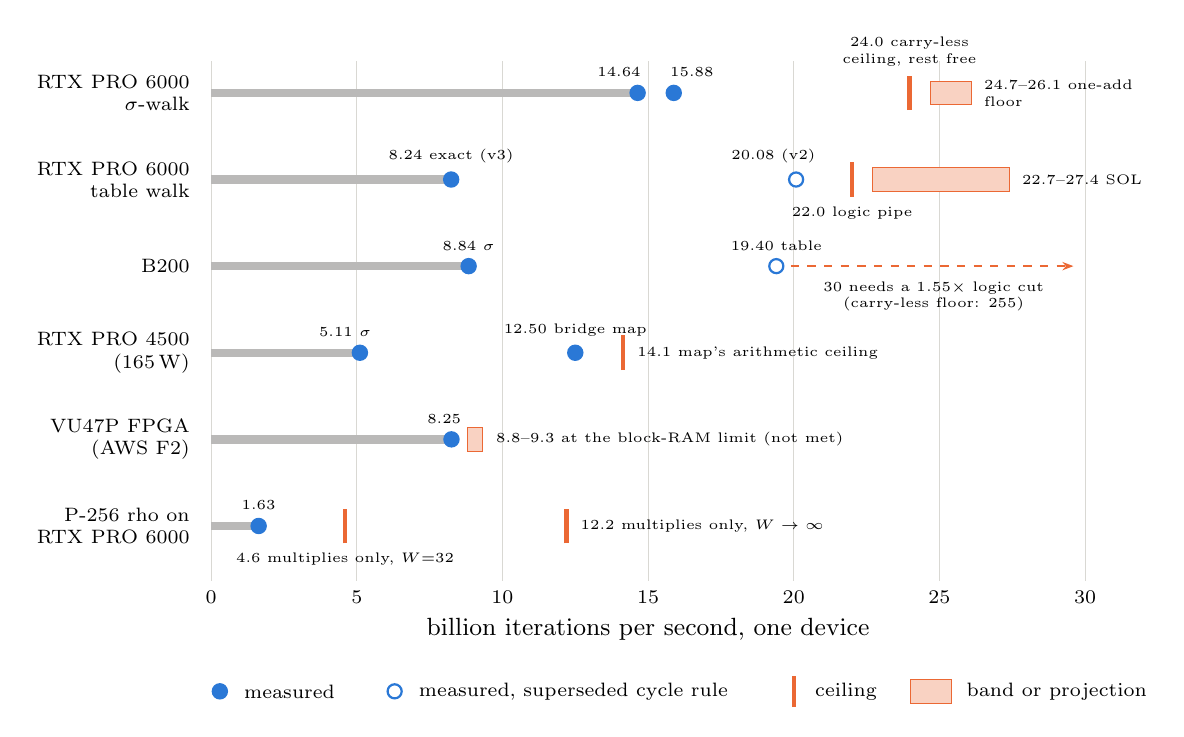
\begin{tikzpicture}[font=\scriptsize,x=0.37cm,y=1cm,
  meas/.style={circle,fill=cA,inner sep=2.1pt},
  old/.style={circle,draw=cA,fill=white,thick,inner sep=1.8pt},
  ceil/.style={draw=cB,line width=1.6pt},
  band/.style={fill=cB!30,draw=cB},
  lab/.style={anchor=east,align=right,font=\scriptsize}]
% grid
\foreach \v in {0,5,10,15,20,25,30}{
  \draw[gridc] (\v,0.4) -- (\v,-6.2);
  \node[below,font=\scriptsize] at (\v,-6.2) {\v};
}
\node[below=10pt,font=\small] at (15,-6.2) {billion iterations per second, one device};
% Row 1: RTX PRO 6000 sigma
\node[lab] at (-0.4,0) {RTX PRO 6000\\$\sigma$-walk};
\draw[inkS!40,line width=3pt] (0,0) -- (14.64,0);
\node[meas] at (14.64,0) {}; \node[meas] at (15.88,0) {};
\node[above,font=\tiny] at (14.0,0.08) {14.64};
\node[above,font=\tiny] at (16.5,0.08) {15.88};
\draw[ceil] (23.97,-0.22) -- (23.97,0.22); \node[above,font=\tiny,align=center] at (23.97,0.22) {24.0 carry-less\\ceiling, rest free};
\fill[band] (24.7,-0.15) rectangle (26.1,0.15);
\node[right,font=\tiny,align=left] at (26.2,0) {24.7--26.1 one-add\\floor};
% Row 2: RTX PRO 6000 table
\node[lab] at (-0.4,-1.1) {RTX PRO 6000\\table walk};
\draw[inkS!40,line width=3pt] (0,-1.1) -- (8.24,-1.1);
\node[meas] at (8.24,-1.1) {}; \node[above,font=\tiny] at (8.24,-1.02) {8.24 exact (v3)};
\node[old] at (20.08,-1.1) {}; \node[above,font=\tiny] at (19.3,-1.02) {20.08 (v2)};
\draw[ceil] (22.0,-1.32) -- (22.0,-0.88); \node[below,font=\tiny] at (22.0,-1.32) {22.0 logic pipe};
\fill[band] (22.7,-1.25) rectangle (27.4,-0.95); \node[right,font=\tiny] at (27.5,-1.1) {22.7--27.4 SOL};
% Row 3: B200
\node[lab] at (-0.4,-2.2) {B200};
\draw[inkS!40,line width=3pt] (0,-2.2) -- (8.84,-2.2);
\node[meas] at (8.84,-2.2) {}; \node[above,font=\tiny] at (8.84,-2.12) {8.84 $\sigma$};
\node[old] at (19.40,-2.2) {}; \node[above,font=\tiny] at (19.40,-2.12) {19.40 table};
\draw[-{Stealth[length=4pt]},dashed,cB,thick] (19.9,-2.2) -- (29.6,-2.2);
\node[below,font=\tiny,align=center] at (24.8,-2.27) {30 needs a $1.55\times$ logic cut\\(carry-less floor: 255)};
% Row 4: RTX PRO 4500
\node[lab] at (-0.4,-3.3) {RTX PRO 4500\\(165\,W)};
\draw[inkS!40,line width=3pt] (0,-3.3) -- (5.107,-3.3);
\node[meas] at (5.107,-3.3) {}; \node[above,font=\tiny] at (4.6,-3.22) {5.11 $\sigma$};
\node[meas] at (12.50,-3.3) {}; \node[above,font=\tiny] at (12.5,-3.22) {12.50 bridge map};
\draw[ceil] (14.14,-3.52) -- (14.14,-3.08); \node[right,font=\tiny] at (14.3,-3.3) {14.1 map's arithmetic ceiling};
% Row 5: FPGA
\node[lab] at (-0.4,-4.4) {VU47P FPGA\\(AWS F2)};
\draw[inkS!40,line width=3pt] (0,-4.4) -- (8.25,-4.4);
\node[meas] at (8.25,-4.4) {}; \node[above,font=\tiny] at (8.0,-4.32) {8.25};
\fill[band] (8.8,-4.55) rectangle (9.3,-4.25); \node[right,font=\tiny] at (9.45,-4.4) {8.8--9.3 at the block-RAM limit (not met)};
% Row 6: NIST
\node[lab] at (-0.4,-5.5) {P-256 rho on\\RTX PRO 6000};
\draw[inkS!40,line width=3pt] (0,-5.5) -- (1.632,-5.5);
\node[meas] at (1.632,-5.5) {}; \node[above,font=\tiny] at (1.632,-5.42) {1.63};
\draw[ceil] (4.6,-5.72) -- (4.6,-5.28); \node[below,font=\tiny] at (4.6,-5.72) {4.6 multiplies only, $W{=}32$};
\draw[ceil] (12.2,-5.72) -- (12.2,-5.28); \node[right,font=\tiny] at (12.35,-5.5) {12.2 multiplies only, $W\to\infty$};
% key
\begin{scope}[shift={(0,-7.6)}]
\node[meas] at (0.3,0) {}; \node[anchor=west] at (0.8,0) {measured};
\node[old] at (6.3,0) {}; \node[anchor=west] at (6.8,0) {measured, superseded cycle rule};
\draw[ceil] (20.0,-0.2) -- (20.0,0.2); \node[anchor=west] at (20.4,0) {ceiling};
\fill[band] (24.0,-0.15) rectangle (25.4,0.15); \node[anchor=west] at (25.6,0) {band or projection};
\end{scope}
\end{tikzpicture}
\caption{How far each platform can go, against what it does today.
  Ceilings are derived from measured pipe rates with every other cost
  set to zero, so they are upper bounds, not targets: the RTX~PRO~6000's
  are its carry-less and logic pipes for any walk with one affine
  addition per step (Section~\ref{sec:floor}); the NIST bounds count only
  field multiplications at the measured multiply rate
  (Section~\ref{sec:bounds-nist}). None of these moves the $2^{60.9}$
  iteration count.}
\label{fig:bounds}
\end{figure}

% Expected days = 2^60.9 / (N R) / 86400 = 24896 / (N R) for R in billion it/s.
% Plotted parametrically in log10(N) so the curves sample evenly on the log axis.
\begin{figure}[t]
\centering
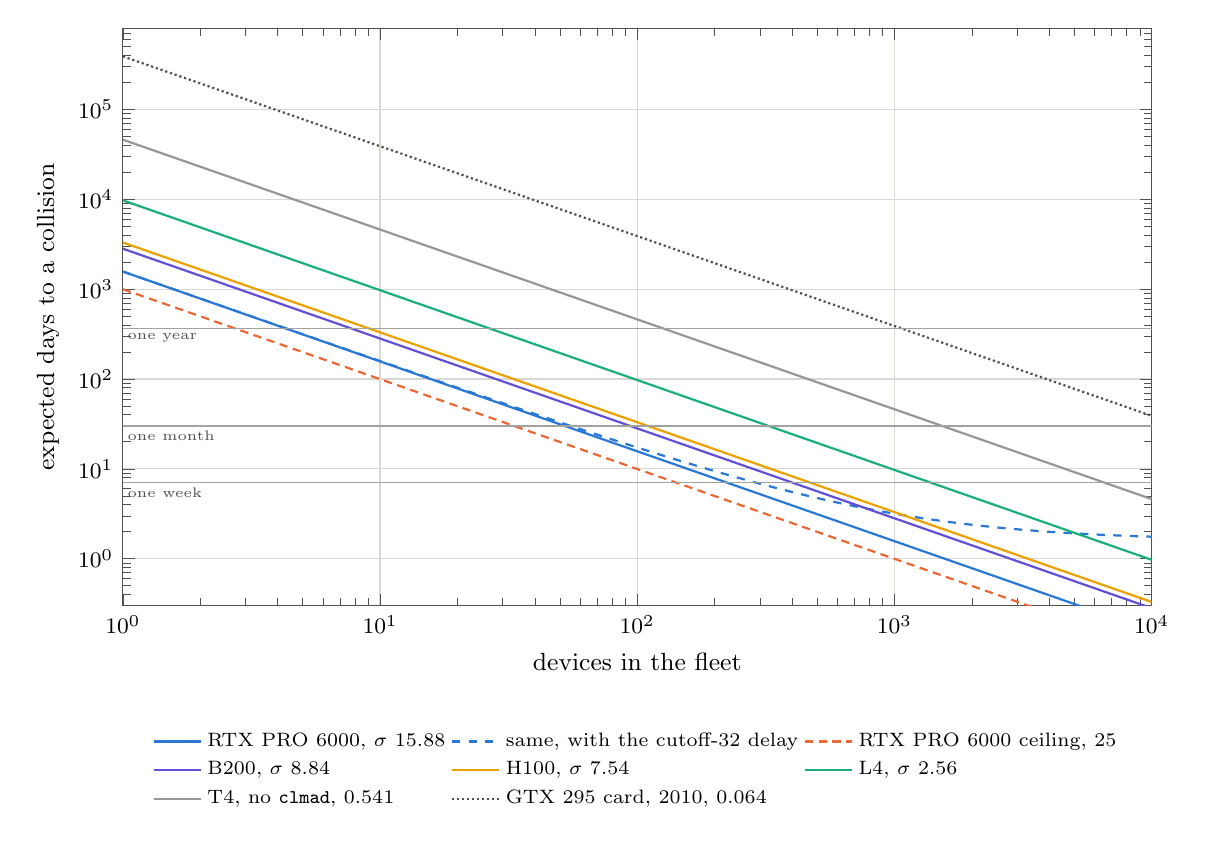
\begin{tikzpicture}
\begin{loglogaxis}[
  width=0.92\textwidth, height=0.56\textwidth,
  xmin=1, xmax=10000, ymin=0.3, ymax=8e5,
  xlabel={devices in the fleet},
  ylabel={expected days to a collision},
  xmajorgrids, ymajorgrids,
  legend style={at={(0.5,-0.2)},anchor=north,font=\scriptsize},
  legend columns=3, legend cell align=left,
  every axis plot/.append style={thick},
]
\addplot[cA,domain=0:4,samples=2] ({10^x},{24896/(15.884*10^x)});
\addlegendentry{RTX PRO 6000, $\sigma$ 15.88}
\addplot[cA,dashed,domain=0:4,samples=60] ({10^x},{24896/(15.884*10^x)+1.6});
\addlegendentry{same, with the cutoff-32 delay}
\addplot[cB,densely dashed,domain=0:4,samples=2] ({10^x},{24896/(25*10^x)});
\addlegendentry{RTX PRO 6000 ceiling, 25}
\addplot[cE,domain=0:4,samples=2] ({10^x},{24896/(8.840*10^x)});
\addlegendentry{B200, $\sigma$ 8.84}
\addplot[cD,domain=0:4,samples=2] ({10^x},{24896/(7.540*10^x)});
\addlegendentry{H100, $\sigma$ 7.54}
\addplot[cC,domain=0:4,samples=2] ({10^x},{24896/(2.561*10^x)});
\addlegendentry{L4, $\sigma$ 2.56}
\addplot[inkS!60,domain=0:4,samples=2] ({10^x},{24896/(0.541*10^x)});
\addlegendentry{T4, no \texttt{clmad}, 0.541}
\addplot[inkS,densely dotted,domain=0:4,samples=2] ({10^x},{24896/(0.064*10^x)});
\addlegendentry{GTX 295 card, 2010, 0.064}
% calendar references
\draw[gridc!60!inkS,line width=0.4pt] (axis cs:1,7) -- (axis cs:10000,7);
\node[anchor=north west,font=\tiny,text=inkS,inner sep=1.5pt] at (axis cs:1,7) {one week};
\draw[gridc!60!inkS,line width=0.4pt] (axis cs:1,30) -- (axis cs:10000,30);
\node[anchor=north west,font=\tiny,text=inkS,inner sep=1.5pt] at (axis cs:1,30) {one month};
\draw[gridc!60!inkS,line width=0.4pt] (axis cs:1,365) -- (axis cs:10000,365);
\node[anchor=north west,font=\tiny,text=inkS,inner sep=1.5pt] at (axis cs:1,365) {one year};
\end{loglogaxis}
\end{tikzpicture}
\caption{Expected calendar time to walk $2^{60.9}$ iterations of
  ECC2K-130 against fleet size, at measured one-device rates in billions
  of iterations per second (Table~\ref{tab:solvetime}), with the 2010
  GTX~295 for comparison. Solid lines count walking time only. The
  dashed line adds the RTX~PRO~6000's detection delay at cutoff 32
  (about $1.6$ days), which sets a floor that more cards cannot lower.
  The median solve is $0.94\times$ the plotted time and the $90\%$
  point $1.71\times$.}
\label{fig:solvetime}
\end{figure}

\end{document}
